\chapter{Generación y Preparación de Datos}

Con el propósito de garantizar la reproducibilidad de los experimentos y proporcionar una base homogénea para todas las implementaciones desarrolladas, el proyecto incorpora un mecanismo automatizado para la generación de datos sintéticos de naturaleza metagenómica.

El procedimiento implementado permite que las versiones Secuencial, Multicore, OpenMP, MPI y CUDA operen exactamente sobre el mismo conjunto de datos de entrada. De esta forma, cualquier diferencia observada durante la experimentación puede atribuirse exclusivamente a la estrategia de paralelización empleada y no a variaciones en los datos procesados.

\section{Objetivo}

El objetivo principal de la generación de datos consiste en construir un conjunto de muestras biológicas sintéticas que permita evaluar el algoritmo de optimización encargado de encontrar el vector de pesos $W$ que maximiza la métrica ROC-AUC.

La utilización de datos sintéticos ofrece las siguientes ventajas:

\begin{itemize}
\item Reproducibilidad de los experimentos.
\item Control completo sobre las características estadísticas del conjunto de datos.
\item Validación funcional del algoritmo.
\item Comparación objetiva entre implementaciones.
\item Escalabilidad mediante la modificación del número de ítems metagenómicos.
\item Independencia respecto a bases de datos biológicas reales.
\end{itemize}

\section{Características del Dataset}

El conjunto de datos generado sigue las especificaciones establecidas en el planteamiento del proyecto.

\begin{itemize}
\item Número total de muestras: 10.
\item Muestras sanas: 5.
\item Muestras enfermas: 5.
\item Número configurable de ítems metagenómicos ($N$).
\item Matriz de contribución $A \in \mathbb{R}^{10\times N}$.
\item Etiquetas binarias $y \in \{0,1\}$.
\item Valores normalizados mediante distribución Dirichlet.
\item Compatibilidad con todas las implementaciones desarrolladas.
\end{itemize}

Las primeras cinco filas de la matriz representan individuos sanos ($y=0$), mientras que las cinco restantes corresponden a individuos enfermos ($y=1$).

\section{Modelo de Representación}

Cada muestra está compuesta por un conjunto de ítems metagenómicos cuya contribución se almacena en la matriz:

\[
A \in \mathbb{R}^{10 \times N}
\]

donde:

\begin{itemize}
\item Cada fila representa una muestra biológica.
\item Cada columna representa un ítem metagenómico.
\item Cada elemento $a_{ij}$ cuantifica la contribución del ítem $i$ en la muestra $j$.
\end{itemize}

La matriz es utilizada posteriormente para calcular:

\[
Score = A \cdot P
\]

donde $P$ corresponde al vector de puntuaciones por ítem obtenido mediante la combinación ponderada de los perfiles taxonómico, ecológico y funcional.

\section{Proceso de Generación}

La generación del conjunto de datos sigue una secuencia de etapas claramente definidas, ilustradas en la Figura \ref{fig:generacion_datos}.

\begin{figure}[H]
\centering
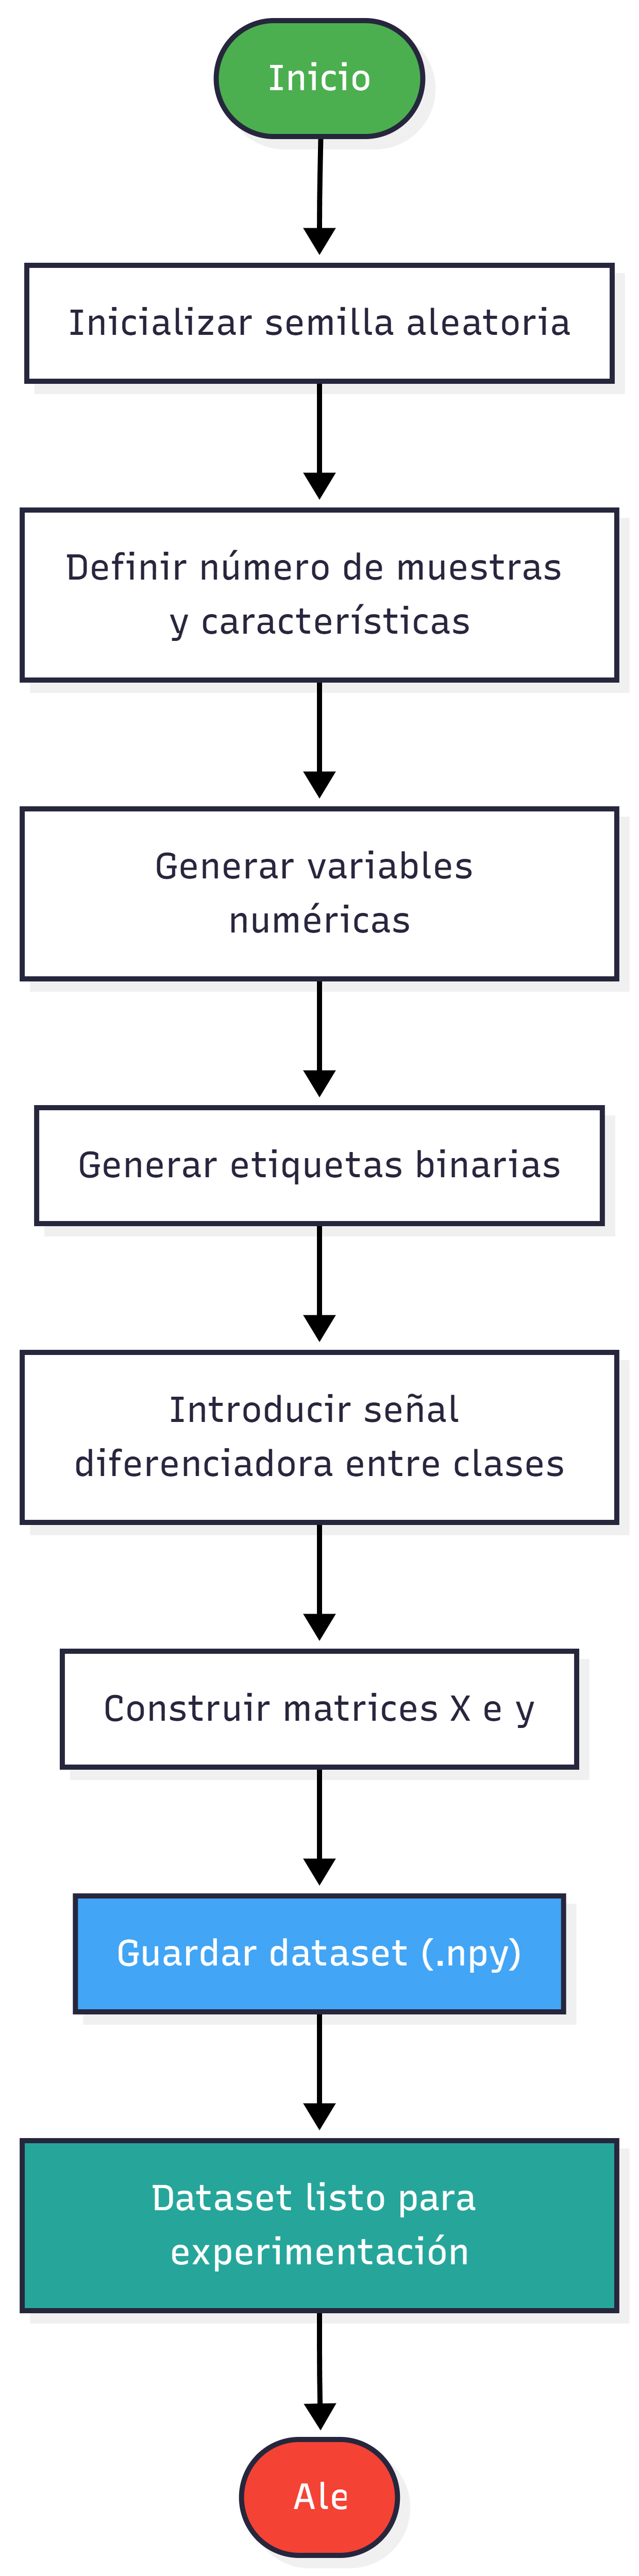
\includegraphics[width=0.90\textwidth,height=0.55\textheight,keepaspectratio]
{figuras/arquitectura/06_generacion_datos.png}
\caption{Proceso de generación del conjunto de datos utilizado durante los experimentos.}
\label{fig:generacion_datos}
\end{figure}

El procedimiento implementado comprende las siguientes etapas:

\begin{enumerate}
\item Inicialización de una semilla aleatoria fija.
\item Definición del número de ítems metagenómicos $N$.
\item Generación de la matriz $A$ mediante una distribución Dirichlet.
\item Construcción de las etiquetas binarias.
\item Asignación de cinco muestras sanas y cinco muestras enfermas.
\item Almacenamiento de la matriz y etiquetas.
\item Disponibilización de los datos para todas las implementaciones.
\end{enumerate}

Este flujo garantiza que cualquier experimento pueda repetirse exactamente bajo las mismas condiciones.

\section{Script de Generación}

La generación del conjunto de datos se realiza mediante el script \texttt{generate\_data.py}, incluido dentro del directorio \texttt{data/}.

\begin{lstlisting}[language=Python, caption={Script de generación de datos}]
import numpy as np

def generate_data(n_items: int = 50, seed: int = 42):
    """
    Genera A en R^(10 x n_items) y etiquetas y.
    Filas 0-4: sanas (y=0).
    Filas 5-9: enfermas (y=1).
    Cada fila de A es Dirichlet(1,...,1).
    """
    rng = np.random.default_rng(seed)

    A = rng.dirichlet(
        np.ones(n_items),
        size=10
    ).astype(np.float32)

    y = np.array(
        [0]*5 + [1]*5,
        dtype=np.int32
    )

    return A, y

if __name__ == "__main__":
    A, y = generate_data(n_items=50)

    np.save("data/matrix_A.npy", A)
    np.save("data/labels.npy", y)

    print(f"A: {A.shape} | y: {y}")
\end{lstlisting}

La parametrización mediante la variable \texttt{n\_items} permite incrementar el tamaño del problema para realizar pruebas de escalabilidad y rendimiento.

\section{Formato de Almacenamiento}

Los datos se almacenan utilizando archivos con extensión \texttt{.npy}, formato binario nativo de NumPy optimizado para matrices multidimensionales.

Los archivos generados son:

\begin{itemize}
\item \texttt{matrix\_A.npy}
\item \texttt{labels.npy}
\end{itemize}

El uso de este formato proporciona:

\begin{itemize}
\item Lectura rápida.
\item Bajo consumo de memoria.
\item Compatibilidad entre implementaciones.
\item Eliminación de conversiones innecesarias.
\item Acceso eficiente desde Python, C y CUDA.
\end{itemize}

\section{Reproducibilidad Experimental}

Para garantizar la repetibilidad de los experimentos, el generador utiliza una semilla fija:

\[
seed = 42
\]

Gracias a este procedimiento, todas las implementaciones procesan exactamente el mismo conjunto de datos, permitiendo realizar comparaciones objetivas de:

\begin{itemize}
\item Tiempo de ejecución.
\item ROC-AUC obtenido.
\item Speedup.
\item Eficiencia.
\item Escalabilidad.
\item Utilización de recursos computacionales.
\end{itemize}

\section{Ejemplo del Dataset}

La Figura \ref{fig:dataset} presenta una vista parcial de la matriz generada automáticamente por el sistema.

\begin{figure}[H]
\centering
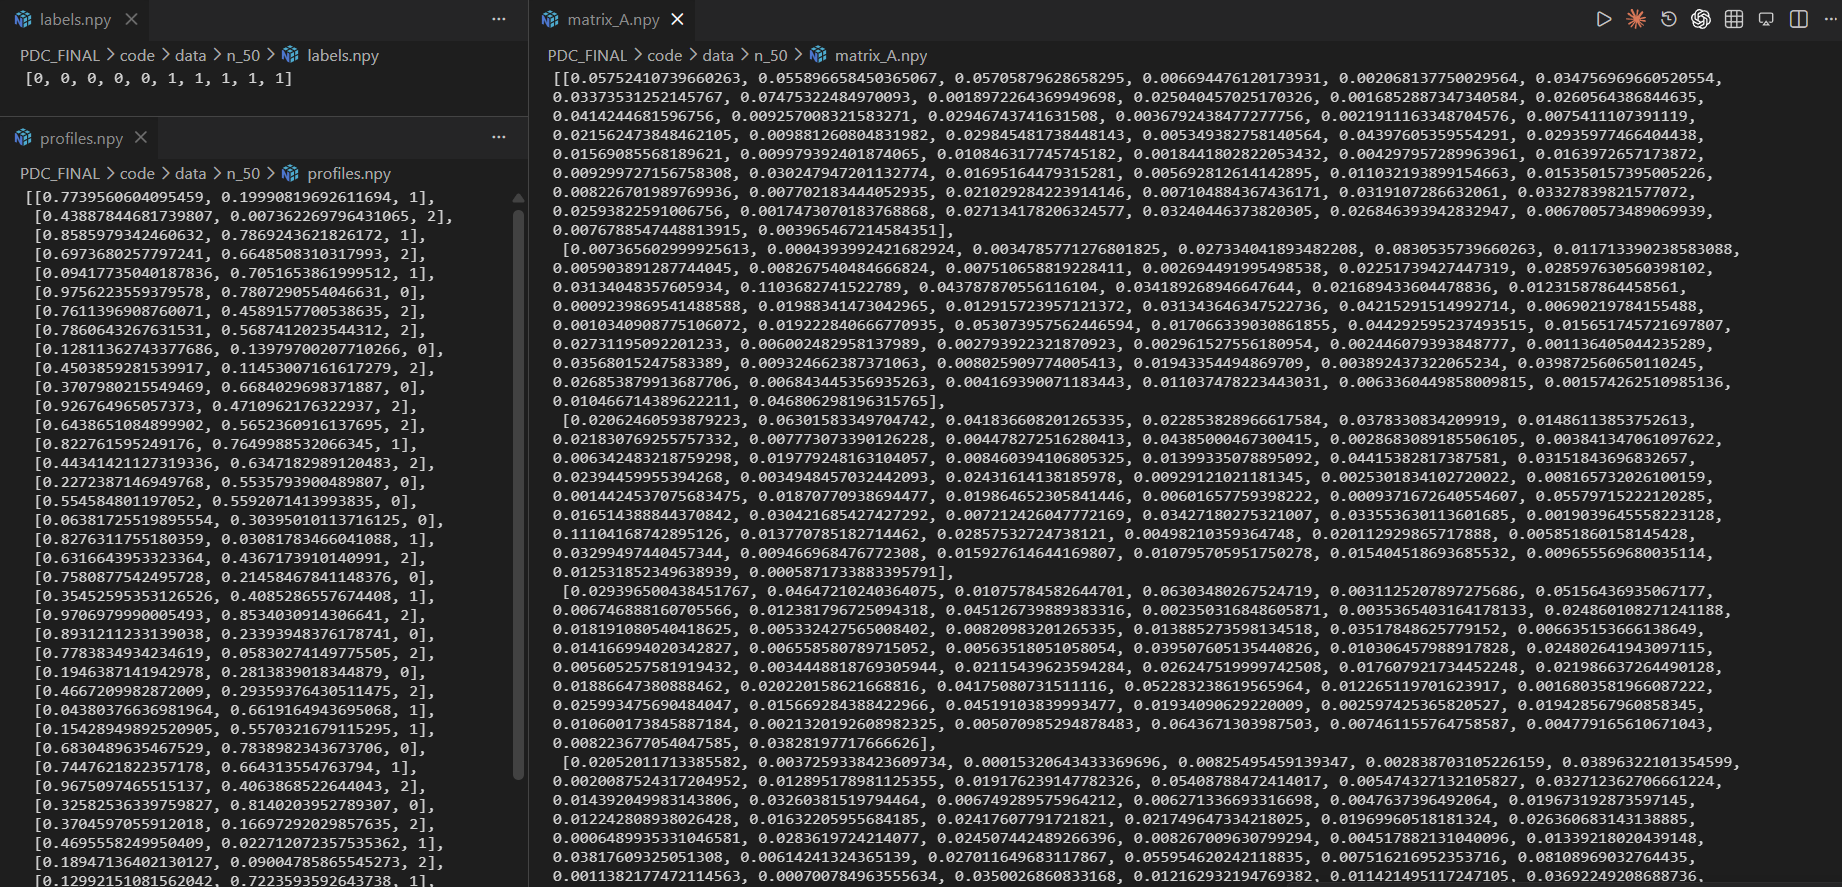
\includegraphics[width=0.92\textwidth,height=0.5\textheight,keepaspectratio]
{figuras/arquitectura/07_dataset_tabla.png}
\caption{Vista parcial de la matriz de contribución utilizada durante los experimentos.}
\label{fig:dataset}
\end{figure}

Cada fila corresponde a una muestra biológica y cada columna representa un ítem metagenómico generado sintéticamente.

\section{Importancia del Dataset}

El uso de un único conjunto de datos garantiza que todas las implementaciones trabajen bajo exactamente las mismas condiciones experimentales.

Esta característica resulta fundamental para evaluar de forma objetiva el impacto de cada paradigma de computación sobre el rendimiento del algoritmo. De esta manera, las diferencias observadas en tiempo de ejecución, speedup, eficiencia y escalabilidad pueden atribuirse exclusivamente a la estrategia de paralelización utilizada y no a modificaciones en los datos de entrada.

Además, la posibilidad de incrementar el número de ítems metagenómicos permite construir escenarios de prueba progresivamente más exigentes, facilitando el estudio del comportamiento del algoritmo en entornos de computación de alto rendimiento.